% This file contains the layout of the first six pages and the explanation text
% of a compilation thesis. 

%%%%%%%%%%%%% FIRST PAGES WITH THESIS TITLE ETC %%%%%%%%%%%%%%%%%%%%%%%%%%%%%%%%
\frontmatter % roman numbers

% Page one: Title only
\thispagestyle{empty} % no page number
\begin{center}
  \vspace*{5cm}
  {\Large \myMainTitle}
  %\\
  %{\large \mySubTitle}
\end{center}

% Page two: empty. Empty space is important

%%%%%%%%%%%%%%%%%%%%%%%%%%%%%%%%%%%%%%%%%%%%%%%%%%%%%%%%%%%%%%%%%%%%%%%
% Page three: title page with small text (spikningsblad)

\cleardoublepage
\thispagestyle{empty} % no page number
~
\vspace*{0.80cm}
\begin{center}
  {\Huge \myMainTitle}
  \\[2mm]
  {\Large \mySubTitle}

  \vspace*{6ex}

  {\Large\myName}

  \vspace*{6ex}
  % black and white (default):
  
\includegraphics[width=0.25\textwidth]{LundUniversity_C2line_BLACK.eps}

  \vspace*{6ex}

  {\large \myDegree}

  \vspace*{6ex}

  {%
    {\small\scshape Thesis Advisors}\\
    \large\myAdvisors
  }

  \bigskip

  {%
    {\small\scshape Faculty Opponent}\\
    \large \myOpponent
  }

  \vspace*{5ex}

  {\footnotesize
    \myDefenceAnnouncement
  }
  \\
\end{center}
\vfill

%%%%%%%%%%%%%%%%%%%%%%%%%%%%%%%%%%%%%%%%%%%%%%%%%%%%%%%%%%%%%%%%%%%%%%%
% Page four: data sheet
\newpage

%Either include datasheet texfile (will be filled in automatically), or a pdf
%containing datasheet (text needs to be already in it, edit
%sheetPDF_editable.pdf). Use one of the next two lines: 
\newcounter{aformdx}
\newcounter{aformdy}
\newcounter{aformx}
\newcounter{aformy}
\newcounter{aformtx}
\newcounter{aformtdx}
\newcounter{aformty}
\def\aformw{358}
\def\aformwhalf{\aformw / 2}
\def\aformwquart{\aformw / 4}
\def\aformwthreeq{\aformw / 4 * 3}
\def\aformh{517}
\def\aformb{23}
\def\aformlinew{0.4pt}
\def\aformrowh{20}
\def\aformRowh{24}
\newcommand\aformhline
{\put(\value{aformx},\value{aformy}){\line(1,0){\value{aformdx}}}}
\newcommand\aformvline
{\put(\value{aformx},\value{aformy}){\line(0,-1){\value{aformdy}}}}
\newcommand\aformvlinec
{\put(\value{aformx},\value{aformy}){\line(0,-1){16.25}}}
\newcommand\aformboxbase[5]
{
  \setcounter{aformtx}{\value{aformx}}
  \setcounter{aformtdx}{\value{aformdx}}
  \setcounter{aformty}{\value{aformy}}
  \addtocounter{aformtx}{#1}
  \addtocounter{aformtdx}{-#2}
  \addtocounter{aformty}{-#3}
  \put(\value{aformtx},\value{aformty})
  {
    \parbox[t]{\value{aformtdx}pt}
    {{\sf\tiny #4}{\scriptsize #5\par}}
  }
}
\newcommand\aformbox[2]{\aformboxbase{2}{11}{8}{#1}{#2}}
\newcommand\aformBox[2]{\aformboxbase{2}{11}{8}{#1}{#2}}

\begin{center}
  \begin{picture}(\aformw,510)(0,0)
    \linethickness{\aformlinew}
    \put(0,\aformb){\framebox(\aformw,\aformh){}}
    \put(-14,200){\rotatebox{90}{\parbox{200pt}
        {\sf\tiny
          DOKUMENTDATABLAD
          enl SIS 61 41 21\\
        }}}
    \setcounter{aformx}{0}
    \setcounter{aformy}{\aformb}
    \addtocounter{aformy}{\aformh}
    \setcounter{aformdx}{\aformwhalf}
    \aformbox{Organization}
    {\\
    {\bf LUND UNIVERSITY}\vspace{0.1cm}
    \\
    {\myDepartment\\
    \myAddress}
    }
    \setcounter{aformdy}{\aformrowh}
    \addtocounter{aformdy}{\aformrowh}
    \addtocounter{aformdy}{\aformrowh}
    \addtocounter{aformdy}{\aformRowh}
    \setcounter{aformx}{\aformwhalf}
    \aformvline
    \setcounter{aformx}{0}
    \addtocounter{aformy}{-\aformrowh}
    \addtocounter{aformy}{-\aformrowh}
    \addtocounter{aformy}{-\aformRowh}
    \aformbox{Author(s)}{\\\myName}
    \setcounter{aformdy}{\aformrowh}
    \aformhline
    \addtocounter{aformy}{\aformrowh}
    \addtocounter{aformy}{\aformrowh}
    \addtocounter{aformy}{\aformRowh}
    \setcounter{aformx}{\aformwhalf}
    \aformbox{Document name}{\\{\bf DOCTORAL DISSERTATION}}
    \addtocounter{aformy}{-\aformrowh}
    \aformhline
    \aformbox{Date of disputation}{\\\myFormDefenceDate}
    \setcounter{aformx}{\aformwhalf}
    \aformhline
    \addtocounter{aformy}{-\aformrowh}
    \addtocounter{aformdy}{\aformRowh}
    \aformbox{Sponsoring organization}{}
    \aformhline
    \addtocounter{aformy}{-\aformRowh}
    \addtocounter{aformy}{-\aformrowh}
    \setcounter{aformx}{0}
    \setcounter{aformdx}{\aformw}
    \aformhline
    \aformbox{Title and subtitle }{\\\myTitle}
    \addtocounter{aformy}{-\aformRowh}
    \setcounter{aformx}{0}
    \aformhline
    \aformBox{Abstract}
    {\\
    {\parskip0pt\parindent1em
    \myAbstract
    }
    }
    \setcounter{aformy}{\aformb}
    % Correspond to one minus each in the bottom section
    \addtocounter{aformy}{\aformRowh}
    \addtocounter{aformy}{\aformRowh}
    \addtocounter{aformy}{\aformRowh}
    \addtocounter{aformy}{\aformRowh}
    \addtocounter{aformy}{\aformrowh}
    \addtocounter{aformy}{\aformrowh}
    \addtocounter{aformy}{10}
    \addtocounter{aformy}{10}
    \aformhline
    \aformbox{Key words}
    {
      \\\myFormKeywords
    }
    \addtocounter{aformy}{-\aformRowh}
    \addtocounter{aformy}{-10}
    \aformhline
    \aformbox{Classification system and/or index terms (if any)}{}
    \addtocounter{aformy}{-\aformRowh}
    \aformhline
    \aformbox{Supplementary bibliographical information}{}
    \setcounter{aformx}{\aformwthreeq}
    \setcounter{aformdx}{\aformwquart}
    \setcounter{aformdy}{\aformRowh}
    \aformvline
    \aformbox{Language}{\\English}
    \addtocounter{aformy}{-\aformRowh}
    \setcounter{aformx}{0}
    \setcounter{aformdx}{\aformw}
    \aformhline
    \aformbox{ISSN and key title}{}
    \setcounter{aformx}{\aformwthreeq}
    \addtocounter{aformdy}{10}
    \aformvline
    \addtocounter{aformdy}{-10}
    \aformbox{ISBN}{\\\myISBNprint\xspace(print)\\\myISBNpdf\xspace(pdf)}
    \addtocounter{aformy}{-\aformRowh}
    \addtocounter{aformy}{-10}
    \setcounter{aformx}{0}
    \aformhline
    \aformbox{Recipient's notes}{}
    \setcounter{aformx}{\aformwhalf}
    \setcounter{aformdy}{\aformrowh}
    \addtocounter{aformdy}{\aformrowh}
    \aformvline
    \aformbox{Number of pages}{\\227}
    \setcounter{aformx}{\aformwthreeq}
    \aformbox{Price}{}
    \setcounter{aformdy}{\aformrowh}
    \aformvline
    \addtocounter{aformy}{-\aformrowh}
    \setcounter{aformx}{\aformwhalf}
    \setcounter{aformdx}{\aformwhalf}
    \aformhline
    \aformbox{Security classification}{}
    \setcounter{aformx}{0}
    \setcounter{aformdx}{\aformw}
    \addtocounter{aformy}{-\aformrowh}
    \addtocounter{aformy}{-4}
    \aformbox{}
    {\scriptsize I, the undersigned, being the copyright owner of the abstract of the
      above-mentioned dissertation, hereby grant to all reference sources
      the permission to publish and disseminate the abstract of the
      above-mentioned dissertation.
    }
    \addtocounter{aformy}{-\aformRowh}
    \addtocounter{aformy}{-20}
    \aformbox{
      \hspace{0pt}
      %\put(44,1){\includegraphics{images/signature}} %Media-Tryck does not want this to be included as a graphic
    }{}
    \aformbox{\rm
      \scriptsize
      Signature \underline{\hskip 140pt}\hfill Date \underline{\hskip 80pt}
    }{}
    \addtocounter{aformy}{1}
    \aformbox{}{\hskip 280pt \scriptsize \myFormSignDate}
  \end{picture}
\end{center}

%\addtocounter{pages}{1} 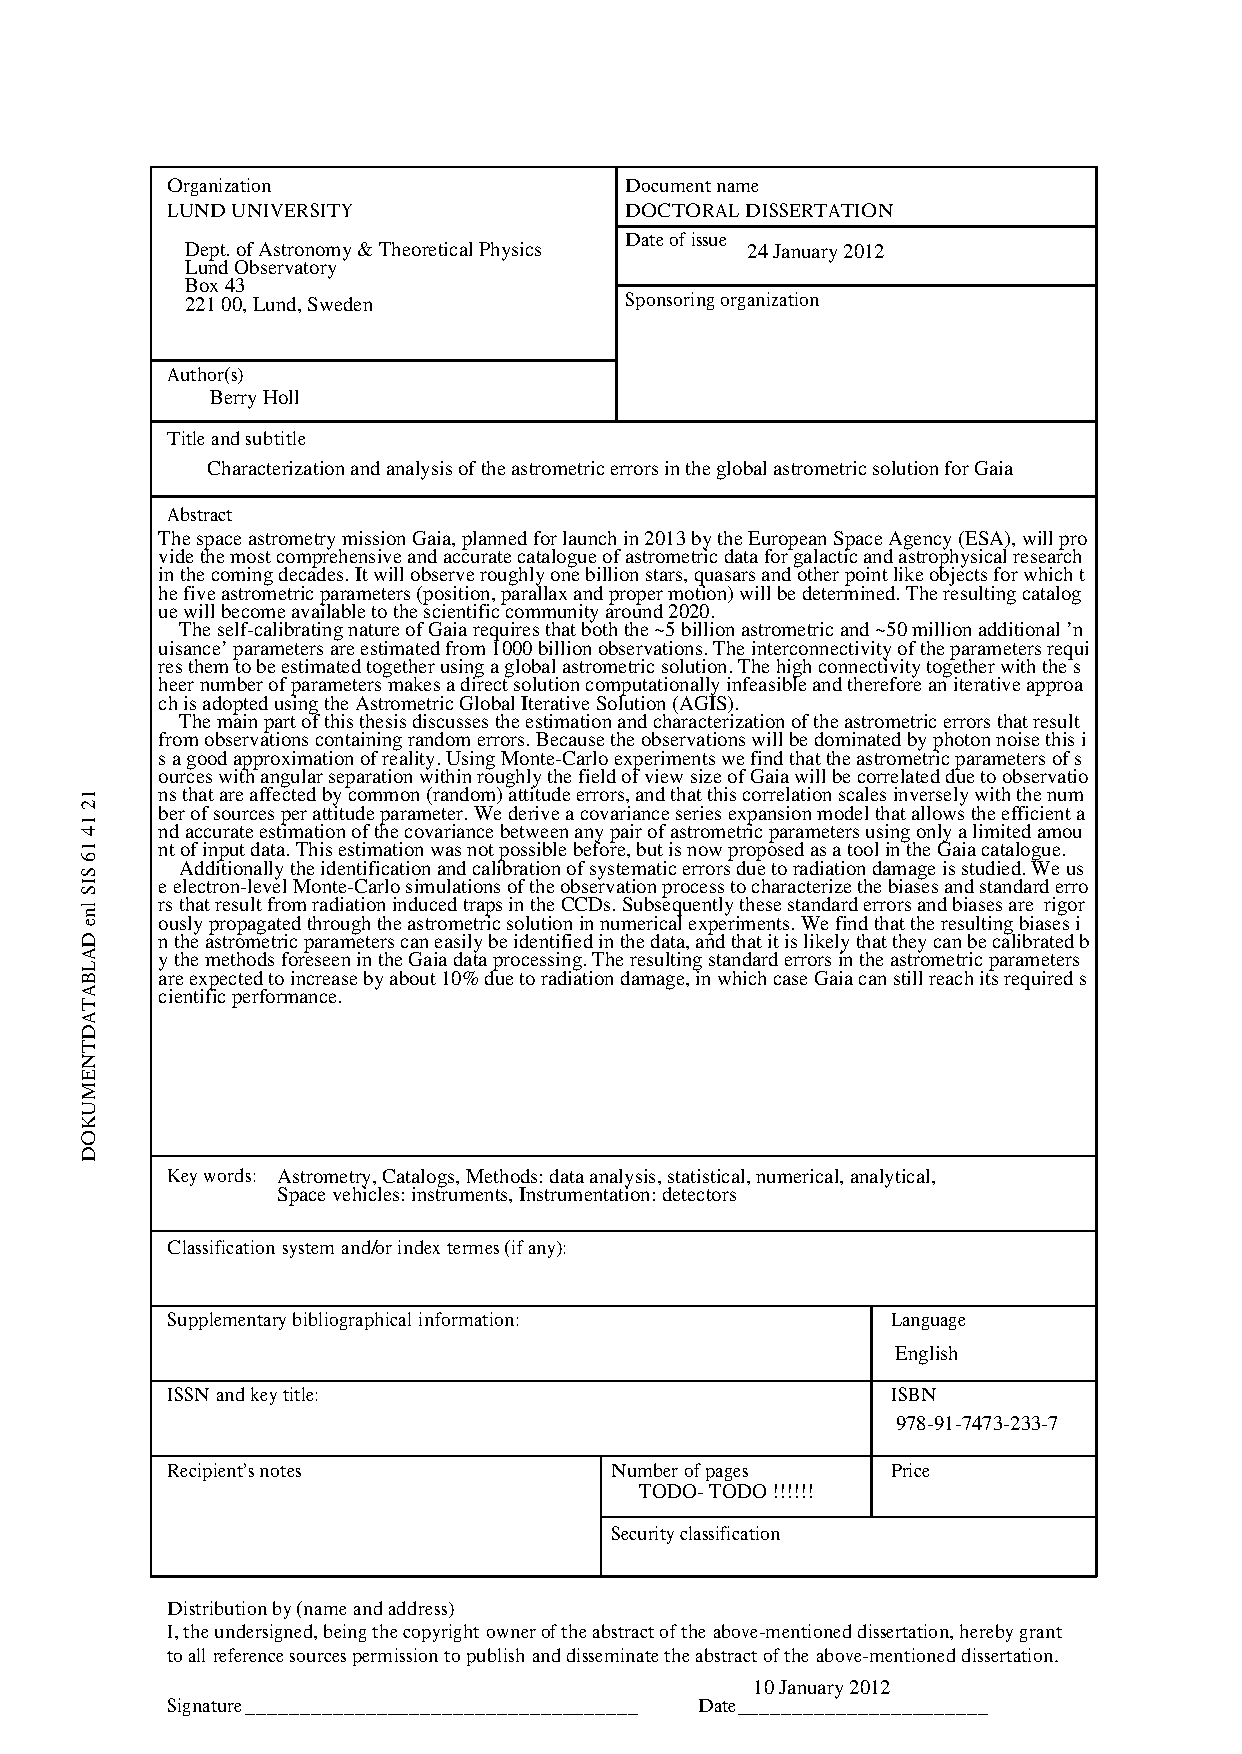
\includepdf[pages=1-1]{datasheetPDF_editable}

%%%%%%%%%%%%%%%%%%%%%%%%%%%%%%%%%%%%%%%%%%%%%%%%%%%%%%%%%%%%%%%%%%%%%%%
% Page five: title and author, without small text. Looks good!

\cleardoublepage
\thispagestyle{empty} % no page number
~
\vspace*{0.80cm}
\begin{center}
  {\Huge \myMainTitle}
  \\[2mm]
  {\Large \mySubTitle}

  \vspace*{6ex}

  {\Large\myName}

  \vspace*{6ex}
  % black and white (default):
  
\includegraphics[width=0.25\textwidth]{LundUniversity_C2line_BLACK.eps}
\end{center}
\vfill


%%%%%%%%%%%%%%%%%%%%%%%%%%%%%%%%%%%%%%%%%%%%%%%%%%%%%%%%%%%%%%%%%%%%%%%
% Page six: Cover image description, ISBN, copyright
\newpage

\thispagestyle{empty} % no page number

\noindent A doctoral thesis at a university in Sweden takes either the form of a single,
cohesive research study (monograph) or a summary of research papers
(compilation thesis), which the doctoral student has written alone or together
with one or several other author(s).

In the latter case the thesis consists of two parts. An introductory text puts
the research work into context and summarizes the main points of the papers.
Then, the research publications themselves are reproduced, together
with a description of the individual contributions of the authors. The
research papers may either have been already published or are manuscripts at
various stages (in press, submitted, or in draft).

\vfill
{\small
  \myCoverFront\\
  \\
  \myCoverBack\\
  \\
  \myFundingInformation


  \vspace{5mm}
  \noindent\copyright\, \myName~\myYear\\
  \\
  \myFaculty, {\myDepartment}
  \\
  \\
  \ISBN: \myISBNprint~(print)\\ % ISBN av svenska ISBN centralen
  \ISBN: \myISBNpdf~(electronic)\\ % ISBN av svenska ISBN centralen
  % \mySeries\\
  \\
  Printed in Sweden by Media-Tryck, Lund~University, Lund~\myYear

  \medskip

  \noindent
\includegraphics[width=0.5\textwidth]{ENG-Miljologotyper-sid-2-BLACK.eps}
}
